% Created by tikzDevice version 0.12.3 on 2020-01-20 17:11:57
% !TEX encoding = UTF-8 Unicode
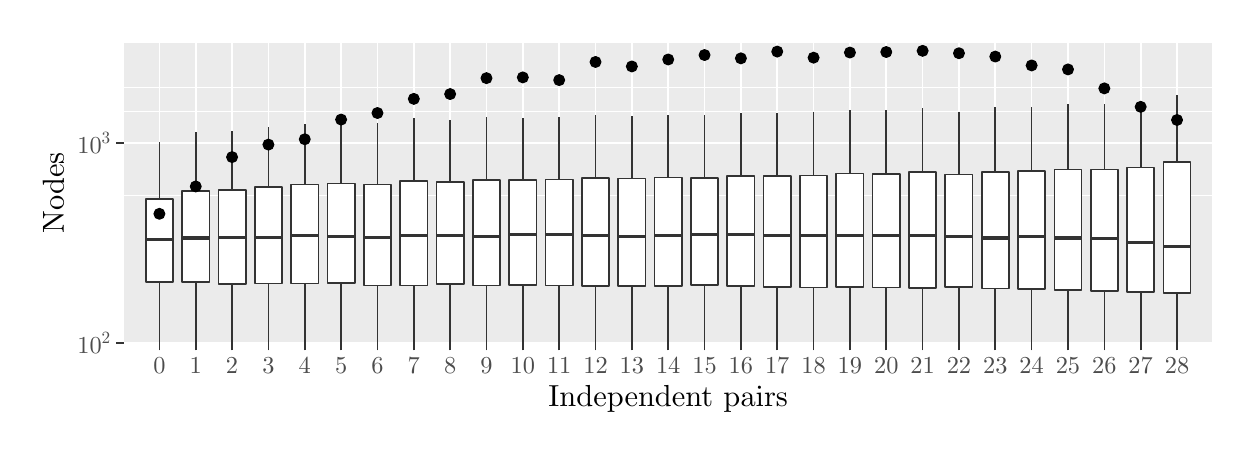
\begin{tikzpicture}[x=1pt,y=1pt]
\definecolor{fillColor}{RGB}{255,255,255}
\path[use as bounding box,fill=fillColor,fill opacity=0.00] (0,0) rectangle (433.62,144.54);
\begin{scope}
\path[clip] (  0.00,  0.00) rectangle (433.62,144.54);
\definecolor{drawColor}{RGB}{255,255,255}
\definecolor{fillColor}{RGB}{255,255,255}

\path[draw=drawColor,line width= 0.6pt,line join=round,line cap=round,fill=fillColor] (  0.00,  0.00) rectangle (433.62,144.54);
\end{scope}
\begin{scope}
\path[clip] ( 34.79, 30.69) rectangle (428.12,139.04);
\definecolor{fillColor}{gray}{0.92}

\path[fill=fillColor] ( 34.79, 30.69) rectangle (428.12,139.04);
\definecolor{drawColor}{RGB}{255,255,255}

\path[draw=drawColor,line width= 0.3pt,line join=round] ( 34.79, 84.06) --
	(428.12, 84.06);

\path[draw=drawColor,line width= 0.3pt,line join=round] ( 34.79,114.41) --
	(428.12,114.41);

\path[draw=drawColor,line width= 0.3pt,line join=round] ( 34.79,122.88) --
	(428.12,122.88);

\path[draw=drawColor,line width= 0.6pt,line join=round] ( 34.79, 30.69) --
	(428.12, 30.69);

\path[draw=drawColor,line width= 0.6pt,line join=round] ( 34.79,102.78) --
	(428.12,102.78);

\path[draw=drawColor,line width= 0.6pt,line join=round] ( 47.60, 30.69) --
	( 47.60,139.04);

\path[draw=drawColor,line width= 0.6pt,line join=round] ( 60.73, 30.69) --
	( 60.73,139.04);

\path[draw=drawColor,line width= 0.6pt,line join=round] ( 73.86, 30.69) --
	( 73.86,139.04);

\path[draw=drawColor,line width= 0.6pt,line join=round] ( 86.99, 30.69) --
	( 86.99,139.04);

\path[draw=drawColor,line width= 0.6pt,line join=round] (100.13, 30.69) --
	(100.13,139.04);

\path[draw=drawColor,line width= 0.6pt,line join=round] (113.26, 30.69) --
	(113.26,139.04);

\path[draw=drawColor,line width= 0.6pt,line join=round] (126.39, 30.69) --
	(126.39,139.04);

\path[draw=drawColor,line width= 0.6pt,line join=round] (139.53, 30.69) --
	(139.53,139.04);

\path[draw=drawColor,line width= 0.6pt,line join=round] (152.66, 30.69) --
	(152.66,139.04);

\path[draw=drawColor,line width= 0.6pt,line join=round] (165.79, 30.69) --
	(165.79,139.04);

\path[draw=drawColor,line width= 0.6pt,line join=round] (178.92, 30.69) --
	(178.92,139.04);

\path[draw=drawColor,line width= 0.6pt,line join=round] (192.06, 30.69) --
	(192.06,139.04);

\path[draw=drawColor,line width= 0.6pt,line join=round] (205.19, 30.69) --
	(205.19,139.04);

\path[draw=drawColor,line width= 0.6pt,line join=round] (218.32, 30.69) --
	(218.32,139.04);

\path[draw=drawColor,line width= 0.6pt,line join=round] (231.46, 30.69) --
	(231.46,139.04);

\path[draw=drawColor,line width= 0.6pt,line join=round] (244.59, 30.69) --
	(244.59,139.04);

\path[draw=drawColor,line width= 0.6pt,line join=round] (257.72, 30.69) --
	(257.72,139.04);

\path[draw=drawColor,line width= 0.6pt,line join=round] (270.85, 30.69) --
	(270.85,139.04);

\path[draw=drawColor,line width= 0.6pt,line join=round] (283.99, 30.69) --
	(283.99,139.04);

\path[draw=drawColor,line width= 0.6pt,line join=round] (297.12, 30.69) --
	(297.12,139.04);

\path[draw=drawColor,line width= 0.6pt,line join=round] (310.25, 30.69) --
	(310.25,139.04);

\path[draw=drawColor,line width= 0.6pt,line join=round] (323.39, 30.69) --
	(323.39,139.04);

\path[draw=drawColor,line width= 0.6pt,line join=round] (336.52, 30.69) --
	(336.52,139.04);

\path[draw=drawColor,line width= 0.6pt,line join=round] (349.65, 30.69) --
	(349.65,139.04);

\path[draw=drawColor,line width= 0.6pt,line join=round] (362.78, 30.69) --
	(362.78,139.04);

\path[draw=drawColor,line width= 0.6pt,line join=round] (375.92, 30.69) --
	(375.92,139.04);

\path[draw=drawColor,line width= 0.6pt,line join=round] (389.05, 30.69) --
	(389.05,139.04);

\path[draw=drawColor,line width= 0.6pt,line join=round] (402.18, 30.69) --
	(402.18,139.04);

\path[draw=drawColor,line width= 0.6pt,line join=round] (415.32, 30.69) --
	(415.32,139.04);
\definecolor{drawColor}{gray}{0.20}

\path[draw=drawColor,line width= 0.6pt,line join=round] ( 47.60, 82.72) --
	( 47.60,103.19);

\path[draw=drawColor,line width= 0.6pt,line join=round] ( 47.60, 52.70) --
	( 47.60, 41.88) --
	( 47.60, 25.23) --
	( 47.60,  0.00);
\definecolor{fillColor}{RGB}{255,255,255}

\path[draw=drawColor,line width= 0.6pt,line join=round,line cap=round,fill=fillColor] ( 42.67, 82.72) --
	( 42.67, 52.70) --
	( 47.60, 52.70) --
	( 52.52, 52.70) --
	( 52.52, 82.72) --
	( 47.60, 82.72) --
	( 42.67, 82.72) --
	cycle;

\path[draw=drawColor,line width= 1.1pt,line join=round] ( 42.67, 67.97) --
	( 47.60, 67.97) --
	( 52.52, 67.97);

\path[draw=drawColor,line width= 0.6pt,line join=round] ( 60.73, 85.45) --
	( 60.73,106.72);

\path[draw=drawColor,line width= 0.6pt,line join=round] ( 60.73, 52.70) --
	( 60.73, 36.00) --
	( 60.73,  0.00);

\path[draw=drawColor,line width= 0.6pt,line join=round,line cap=round,fill=fillColor] ( 55.80, 85.45) --
	( 55.80, 52.70) --
	( 60.73, 52.70) --
	( 65.65, 52.70) --
	( 65.65, 85.45) --
	( 60.73, 85.45) --
	( 55.80, 85.45) --
	cycle;

\path[draw=drawColor,line width= 1.1pt,line join=round] ( 55.80, 68.54) --
	( 60.73, 68.54) --
	( 65.65, 68.54);

\path[draw=drawColor,line width= 0.6pt,line join=round] ( 73.86, 85.83) --
	( 73.86,107.32);

\path[draw=drawColor,line width= 0.6pt,line join=round] ( 73.86, 51.92) --
	( 73.86, 34.23) --
	( 73.86,  0.00);

\path[draw=drawColor,line width= 0.6pt,line join=round,line cap=round,fill=fillColor] ( 68.94, 85.83) --
	( 68.94, 51.92) --
	( 73.86, 51.92) --
	( 78.79, 51.92) --
	( 78.79, 85.83) --
	( 73.86, 85.83) --
	( 68.94, 85.83) --
	cycle;

\path[draw=drawColor,line width= 1.1pt,line join=round] ( 68.94, 68.82) --
	( 73.86, 68.82) --
	( 78.79, 68.82);

\path[draw=drawColor,line width= 0.6pt,line join=round] ( 86.99, 86.94) --
	( 86.99,108.75);

\path[draw=drawColor,line width= 0.6pt,line join=round] ( 86.99, 52.07) --
	( 86.99, 34.79) --
	( 86.99,  0.00);

\path[draw=drawColor,line width= 0.6pt,line join=round,line cap=round,fill=fillColor] ( 82.07, 86.94) --
	( 82.07, 52.07) --
	( 86.99, 52.07) --
	( 91.92, 52.07) --
	( 91.92, 86.94) --
	( 86.99, 86.94) --
	( 82.07, 86.94) --
	cycle;

\path[draw=drawColor,line width= 1.1pt,line join=round] ( 82.07, 68.82) --
	( 86.99, 68.82) --
	( 91.92, 68.82);

\path[draw=drawColor,line width= 0.6pt,line join=round] (100.13, 87.86) --
	(100.13,109.89);

\path[draw=drawColor,line width= 0.6pt,line join=round] (100.13, 52.07) --
	(100.13, 34.79) --
	(100.13,  0.00);

\path[draw=drawColor,line width= 0.6pt,line join=round,line cap=round,fill=fillColor] ( 95.20, 87.86) --
	( 95.20, 52.07) --
	(100.13, 52.07) --
	(105.05, 52.07) --
	(105.05, 87.86) --
	(100.13, 87.86) --
	( 95.20, 87.86) --
	cycle;

\path[draw=drawColor,line width= 1.1pt,line join=round] ( 95.20, 69.46) --
	(100.13, 69.46) --
	(105.05, 69.46);

\path[draw=drawColor,line width= 0.6pt,line join=round] (113.26, 88.21) --
	(113.26,110.29);

\path[draw=drawColor,line width= 0.6pt,line join=round] (113.26, 52.23) --
	(113.26, 34.65) --
	(113.26,  0.00);

\path[draw=drawColor,line width= 0.6pt,line join=round,line cap=round,fill=fillColor] (108.34, 88.21) --
	(108.34, 52.23) --
	(113.26, 52.23) --
	(118.18, 52.23) --
	(118.18, 88.21) --
	(113.26, 88.21) --
	(108.34, 88.21) --
	cycle;

\path[draw=drawColor,line width= 1.1pt,line join=round] (108.34, 69.19) --
	(113.26, 69.19) --
	(118.18, 69.19);

\path[draw=drawColor,line width= 0.6pt,line join=round] (126.39, 87.91) --
	(126.39,110.12);

\path[draw=drawColor,line width= 0.6pt,line join=round] (126.39, 51.43) --
	(126.39, 34.23) --
	(126.39,  0.00);

\path[draw=drawColor,line width= 0.6pt,line join=round,line cap=round,fill=fillColor] (121.47, 87.91) --
	(121.47, 51.43) --
	(126.39, 51.43) --
	(131.32, 51.43) --
	(131.32, 87.91) --
	(126.39, 87.91) --
	(121.47, 87.91) --
	cycle;

\path[draw=drawColor,line width= 1.1pt,line join=round] (121.47, 68.82) --
	(126.39, 68.82) --
	(131.32, 68.82);

\path[draw=drawColor,line width= 0.6pt,line join=round] (139.53, 89.24) --
	(139.53,111.73);

\path[draw=drawColor,line width= 0.6pt,line join=round] (139.53, 51.43) --
	(139.53, 34.51) --
	(139.53,  0.00);

\path[draw=drawColor,line width= 0.6pt,line join=round,line cap=round,fill=fillColor] (134.60, 89.24) --
	(134.60, 51.43) --
	(139.53, 51.43) --
	(144.45, 51.43) --
	(144.45, 89.24) --
	(139.53, 89.24) --
	(134.60, 89.24) --
	cycle;

\path[draw=drawColor,line width= 1.1pt,line join=round] (134.60, 69.28) --
	(139.53, 69.28) --
	(144.45, 69.28);

\path[draw=drawColor,line width= 0.6pt,line join=round] (152.66, 88.81) --
	(152.66,111.09);

\path[draw=drawColor,line width= 0.6pt,line join=round] (152.66, 51.92) --
	(152.66, 35.33) --
	(152.66,  0.00);

\path[draw=drawColor,line width= 0.6pt,line join=round,line cap=round,fill=fillColor] (147.73, 88.81) --
	(147.73, 51.92) --
	(152.66, 51.92) --
	(157.58, 51.92) --
	(157.58, 88.81) --
	(152.66, 88.81) --
	(147.73, 88.81) --
	cycle;

\path[draw=drawColor,line width= 1.1pt,line join=round] (147.73, 69.37) --
	(152.66, 69.37) --
	(157.58, 69.37);

\path[draw=drawColor,line width= 0.6pt,line join=round] (165.79, 89.53) --
	(165.79,112.08);

\path[draw=drawColor,line width= 0.6pt,line join=round] (165.79, 51.43) --
	(165.79, 34.09) --
	(165.79,  0.00);

\path[draw=drawColor,line width= 0.6pt,line join=round,line cap=round,fill=fillColor] (160.87, 89.53) --
	(160.87, 51.43) --
	(165.79, 51.43) --
	(170.72, 51.43) --
	(170.72, 89.53) --
	(165.79, 89.53) --
	(160.87, 89.53) --
	cycle;

\path[draw=drawColor,line width= 1.1pt,line join=round] (160.87, 69.19) --
	(165.79, 69.19) --
	(170.72, 69.19);

\path[draw=drawColor,line width= 0.6pt,line join=round] (178.92, 89.53) --
	(178.92,111.94);

\path[draw=drawColor,line width= 0.6pt,line join=round] (178.92, 51.60) --
	(178.92, 40.77) --
	(178.92, 24.09) --
	(178.92,  0.00);

\path[draw=drawColor,line width= 0.6pt,line join=round,line cap=round,fill=fillColor] (174.00, 89.53) --
	(174.00, 51.60) --
	(178.92, 51.60) --
	(183.85, 51.60) --
	(183.85, 89.53) --
	(178.92, 89.53) --
	(174.00, 89.53) --
	cycle;

\path[draw=drawColor,line width= 1.1pt,line join=round] (174.00, 69.64) --
	(178.92, 69.64) --
	(183.85, 69.64);

\path[draw=drawColor,line width= 0.6pt,line join=round] (192.06, 89.63) --
	(192.06,112.20);

\path[draw=drawColor,line width= 0.6pt,line join=round] (192.06, 51.43) --
	(192.06, 34.51) --
	(192.06,  0.00);

\path[draw=drawColor,line width= 0.6pt,line join=round,line cap=round,fill=fillColor] (187.13, 89.63) --
	(187.13, 51.43) --
	(192.06, 51.43) --
	(196.98, 51.43) --
	(196.98, 89.63) --
	(192.06, 89.63) --
	(187.13, 89.63) --
	cycle;

\path[draw=drawColor,line width= 1.1pt,line join=round] (187.13, 69.64) --
	(192.06, 69.64) --
	(196.98, 69.64);

\path[draw=drawColor,line width= 0.6pt,line join=round] (205.19, 90.11) --
	(205.19,112.82);

\path[draw=drawColor,line width= 0.6pt,line join=round] (205.19, 51.27) --
	(205.19, 33.95) --
	(205.19,  0.00);

\path[draw=drawColor,line width= 0.6pt,line join=round,line cap=round,fill=fillColor] (200.27, 90.11) --
	(200.27, 51.27) --
	(205.19, 51.27) --
	(210.11, 51.27) --
	(210.11, 90.11) --
	(205.19, 90.11) --
	(200.27, 90.11) --
	cycle;

\path[draw=drawColor,line width= 1.1pt,line join=round] (200.27, 69.37) --
	(205.19, 69.37) --
	(210.11, 69.37);

\path[draw=drawColor,line width= 0.6pt,line join=round] (218.32, 90.05) --
	(218.32,112.77);

\path[draw=drawColor,line width= 0.6pt,line join=round] (218.32, 51.11) --
	(218.32, 34.09) --
	(218.32,  0.00);

\path[draw=drawColor,line width= 0.6pt,line join=round,line cap=round,fill=fillColor] (213.40, 90.05) --
	(213.40, 51.11) --
	(218.32, 51.11) --
	(223.25, 51.11) --
	(223.25, 90.05) --
	(218.32, 90.05) --
	(213.40, 90.05) --
	cycle;

\path[draw=drawColor,line width= 1.1pt,line join=round] (213.40, 69.00) --
	(218.32, 69.00) --
	(223.25, 69.00);

\path[draw=drawColor,line width= 0.6pt,line join=round] (231.46, 90.34) --
	(231.46,112.98);

\path[draw=drawColor,line width= 0.6pt,line join=round] (231.46, 51.27) --
	(231.46, 34.51) --
	(231.46,  0.00);

\path[draw=drawColor,line width= 0.6pt,line join=round,line cap=round,fill=fillColor] (226.53, 90.34) --
	(226.53, 51.27) --
	(231.46, 51.27) --
	(236.38, 51.27) --
	(236.38, 90.34) --
	(231.46, 90.34) --
	(226.53, 90.34) --
	cycle;

\path[draw=drawColor,line width= 1.1pt,line join=round] (226.53, 69.37) --
	(231.46, 69.37) --
	(236.38, 69.37);

\path[draw=drawColor,line width= 0.6pt,line join=round] (244.59, 90.24) --
	(244.59,112.89);

\path[draw=drawColor,line width= 0.6pt,line join=round] (244.59, 51.60) --
	(244.59, 34.79) --
	(244.59,  0.00);

\path[draw=drawColor,line width= 0.6pt,line join=round,line cap=round,fill=fillColor] (239.66, 90.24) --
	(239.66, 51.60) --
	(244.59, 51.60) --
	(249.51, 51.60) --
	(249.51, 90.24) --
	(244.59, 90.24) --
	(239.66, 90.24) --
	cycle;

\path[draw=drawColor,line width= 1.1pt,line join=round] (239.66, 69.64) --
	(244.59, 69.64) --
	(249.51, 69.64);

\path[draw=drawColor,line width= 0.6pt,line join=round] (257.72, 90.95) --
	(257.72,113.87);

\path[draw=drawColor,line width= 0.6pt,line join=round] (257.72, 51.11) --
	(257.72, 33.95) --
	(257.72,  0.00);

\path[draw=drawColor,line width= 0.6pt,line join=round,line cap=round,fill=fillColor] (252.80, 90.95) --
	(252.80, 51.11) --
	(257.72, 51.11) --
	(262.65, 51.11) --
	(262.65, 90.95) --
	(257.72, 90.95) --
	(252.80, 90.95) --
	cycle;

\path[draw=drawColor,line width= 1.1pt,line join=round] (252.80, 69.69) --
	(257.72, 69.69) --
	(262.65, 69.69);

\path[draw=drawColor,line width= 0.6pt,line join=round] (270.85, 90.86) --
	(270.85,113.74);

\path[draw=drawColor,line width= 0.6pt,line join=round] (270.85, 50.95) --
	(270.85, 34.51) --
	(270.85,  0.00);

\path[draw=drawColor,line width= 0.6pt,line join=round,line cap=round,fill=fillColor] (265.93, 90.86) --
	(265.93, 50.95) --
	(270.85, 50.95) --
	(275.78, 50.95) --
	(275.78, 90.86) --
	(270.85, 90.86) --
	(265.93, 90.86) --
	cycle;

\path[draw=drawColor,line width= 1.1pt,line join=round] (265.93, 69.37) --
	(270.85, 69.37) --
	(275.78, 69.37);

\path[draw=drawColor,line width= 0.6pt,line join=round] (283.99, 91.13) --
	(283.99,114.18);

\path[draw=drawColor,line width= 0.6pt,line join=round] (283.99, 50.62) --
	(283.99, 33.67) --
	(283.99,  0.00);

\path[draw=drawColor,line width= 0.6pt,line join=round,line cap=round,fill=fillColor] (279.06, 91.13) --
	(279.06, 50.62) --
	(283.99, 50.62) --
	(288.91, 50.62) --
	(288.91, 91.13) --
	(283.99, 91.13) --
	(279.06, 91.13) --
	cycle;

\path[draw=drawColor,line width= 1.1pt,line join=round] (279.06, 69.28) --
	(283.99, 69.28) --
	(288.91, 69.28);

\path[draw=drawColor,line width= 0.6pt,line join=round] (297.12, 91.84) --
	(297.12,114.91);

\path[draw=drawColor,line width= 0.6pt,line join=round] (297.12, 50.95) --
	(297.12, 33.95) --
	(297.12,  0.00);

\path[draw=drawColor,line width= 0.6pt,line join=round,line cap=round,fill=fillColor] (292.20, 91.84) --
	(292.20, 50.95) --
	(297.12, 50.95) --
	(302.04, 50.95) --
	(302.04, 91.84) --
	(297.12, 91.84) --
	(292.20, 91.84) --
	cycle;

\path[draw=drawColor,line width= 1.1pt,line join=round] (292.20, 69.46) --
	(297.12, 69.46) --
	(302.04, 69.46);

\path[draw=drawColor,line width= 0.6pt,line join=round] (310.25, 91.71) --
	(310.25,114.84);

\path[draw=drawColor,line width= 0.6pt,line join=round] (310.25, 50.62) --
	(310.25, 33.24) --
	(310.25,  0.00);

\path[draw=drawColor,line width= 0.6pt,line join=round,line cap=round,fill=fillColor] (305.33, 91.71) --
	(305.33, 50.62) --
	(310.25, 50.62) --
	(315.18, 50.62) --
	(315.18, 91.71) --
	(310.25, 91.71) --
	(305.33, 91.71) --
	cycle;

\path[draw=drawColor,line width= 1.1pt,line join=round] (305.33, 69.28) --
	(310.25, 69.28) --
	(315.18, 69.28);

\path[draw=drawColor,line width= 0.6pt,line join=round] (323.39, 92.36) --
	(323.39,115.64);

\path[draw=drawColor,line width= 0.6pt,line join=round] (323.39, 50.45) --
	(323.39, 33.24) --
	(323.39,  0.00);

\path[draw=drawColor,line width= 0.6pt,line join=round,line cap=round,fill=fillColor] (318.46, 92.36) --
	(318.46, 50.45) --
	(323.39, 50.45) --
	(328.31, 50.45) --
	(328.31, 92.36) --
	(323.39, 92.36) --
	(318.46, 92.36) --
	cycle;

\path[draw=drawColor,line width= 1.1pt,line join=round] (318.46, 69.28) --
	(323.39, 69.28) --
	(328.31, 69.28);

\path[draw=drawColor,line width= 0.6pt,line join=round] (336.52, 91.48) --
	(336.52,114.11);

\path[draw=drawColor,line width= 0.6pt,line join=round] (336.52, 50.78) --
	(336.52, 33.95) --
	(336.52,  0.00);

\path[draw=drawColor,line width= 0.6pt,line join=round,line cap=round,fill=fillColor] (331.59, 91.48) --
	(331.59, 50.78) --
	(336.52, 50.78) --
	(341.44, 50.78) --
	(341.44, 91.48) --
	(336.52, 91.48) --
	(331.59, 91.48) --
	cycle;

\path[draw=drawColor,line width= 1.1pt,line join=round] (331.59, 69.09) --
	(336.52, 69.09) --
	(341.44, 69.09);

\path[draw=drawColor,line width= 0.6pt,line join=round] (349.65, 92.41) --
	(349.65,115.75);

\path[draw=drawColor,line width= 0.6pt,line join=round] (349.65, 50.28) --
	(349.65, 33.38) --
	(349.65,  0.00);

\path[draw=drawColor,line width= 0.6pt,line join=round,line cap=round,fill=fillColor] (344.73, 92.41) --
	(344.73, 50.28) --
	(349.65, 50.28) --
	(354.58, 50.28) --
	(354.58, 92.41) --
	(349.65, 92.41) --
	(344.73, 92.41) --
	cycle;

\path[draw=drawColor,line width= 1.1pt,line join=round] (344.73, 68.54) --
	(349.65, 68.54) --
	(354.58, 68.54);

\path[draw=drawColor,line width= 0.6pt,line join=round] (362.78, 92.67) --
	(362.78,115.95);

\path[draw=drawColor,line width= 0.6pt,line join=round] (362.78, 50.12) --
	(362.78, 33.24) --
	(362.78,  0.00);

\path[draw=drawColor,line width= 0.6pt,line join=round,line cap=round,fill=fillColor] (357.86, 92.67) --
	(357.86, 50.12) --
	(362.78, 50.12) --
	(367.71, 50.12) --
	(367.71, 92.67) --
	(362.78, 92.67) --
	(357.86, 92.67) --
	cycle;

\path[draw=drawColor,line width= 1.1pt,line join=round] (357.86, 68.91) --
	(362.78, 68.91) --
	(367.71, 68.91);

\path[draw=drawColor,line width= 0.6pt,line join=round] (375.92, 93.23) --
	(375.92,116.80);

\path[draw=drawColor,line width= 0.6pt,line join=round] (375.92, 49.78) --
	(375.92, 33.67) --
	(375.92,  0.00);

\path[draw=drawColor,line width= 0.6pt,line join=round,line cap=round,fill=fillColor] (370.99, 93.23) --
	(370.99, 78.50) --
	(370.99, 49.78) --
	(375.92, 49.78) --
	(380.84, 49.78) --
	(380.84, 78.50) --
	(380.84, 93.23) --
	(375.92, 93.23) --
	(370.99, 93.23) --
	cycle;

\path[draw=drawColor,line width= 1.1pt,line join=round] (370.99, 68.54) --
	(375.92, 68.54) --
	(380.84, 68.54);

\path[draw=drawColor,line width= 0.6pt,line join=round] (389.05, 93.35) --
	(389.05,117.00);

\path[draw=drawColor,line width= 0.6pt,line join=round] (389.05, 49.44) --
	(389.05, 32.36) --
	(389.05,  0.00);

\path[draw=drawColor,line width= 0.6pt,line join=round,line cap=round,fill=fillColor] (384.12, 93.35) --
	(384.12, 78.54) --
	(384.12, 49.44) --
	(389.05, 49.44) --
	(393.97, 49.44) --
	(393.97, 78.54) --
	(393.97, 93.35) --
	(389.05, 93.35) --
	(384.12, 93.35) --
	cycle;

\path[draw=drawColor,line width= 1.1pt,line join=round] (384.12, 68.35) --
	(389.05, 68.35) --
	(393.97, 68.35);

\path[draw=drawColor,line width= 0.6pt,line join=round] (402.18, 94.07) --
	(402.18,117.92);

\path[draw=drawColor,line width= 0.6pt,line join=round] (402.18, 49.09) --
	(402.18, 32.51) --
	(402.18,  0.00);

\path[draw=drawColor,line width= 0.6pt,line join=round,line cap=round,fill=fillColor] (397.26, 94.07) --
	(397.26, 79.05) --
	(397.26, 49.09) --
	(402.18, 49.09) --
	(407.11, 49.09) --
	(407.11, 79.05) --
	(407.11, 94.07) --
	(402.18, 94.07) --
	(397.26, 94.07) --
	cycle;

\path[draw=drawColor,line width= 1.1pt,line join=round] (397.26, 67.01) --
	(402.18, 67.01) --
	(407.11, 67.01);

\path[draw=drawColor,line width= 0.6pt,line join=round] (415.32, 95.91) --
	(415.32,120.16);

\path[draw=drawColor,line width= 0.6pt,line join=round] (415.32, 48.56) --
	(415.32, 31.76) --
	(415.32,  0.00);

\path[draw=drawColor,line width= 0.6pt,line join=round,line cap=round,fill=fillColor] (410.39, 95.91) --
	(410.39, 80.45) --
	(410.39, 48.56) --
	(415.32, 48.56) --
	(420.24, 48.56) --
	(420.24, 80.45) --
	(420.24, 95.91) --
	(415.32, 95.91) --
	(410.39, 95.91) --
	cycle;

\path[draw=drawColor,line width= 1.1pt,line join=round] (410.39, 65.50) --
	(415.32, 65.50) --
	(420.24, 65.50);
\definecolor{drawColor}{RGB}{0,0,0}
\definecolor{fillColor}{RGB}{0,0,0}

\path[draw=drawColor,line width= 0.4pt,line join=round,line cap=round,fill=fillColor] ( 47.60, 77.28) circle (  1.96);

\path[draw=drawColor,line width= 0.4pt,line join=round,line cap=round,fill=fillColor] ( 60.73, 87.17) circle (  1.96);

\path[draw=drawColor,line width= 0.4pt,line join=round,line cap=round,fill=fillColor] ( 73.86, 97.77) circle (  1.96);

\path[draw=drawColor,line width= 0.4pt,line join=round,line cap=round,fill=fillColor] ( 86.99,102.29) circle (  1.96);

\path[draw=drawColor,line width= 0.4pt,line join=round,line cap=round,fill=fillColor] (100.13,104.22) circle (  1.96);

\path[draw=drawColor,line width= 0.4pt,line join=round,line cap=round,fill=fillColor] (113.26,111.33) circle (  1.96);

\path[draw=drawColor,line width= 0.4pt,line join=round,line cap=round,fill=fillColor] (126.39,113.70) circle (  1.96);

\path[draw=drawColor,line width= 0.4pt,line join=round,line cap=round,fill=fillColor] (139.53,118.81) circle (  1.96);

\path[draw=drawColor,line width= 0.4pt,line join=round,line cap=round,fill=fillColor] (152.66,120.55) circle (  1.96);

\path[draw=drawColor,line width= 0.4pt,line join=round,line cap=round,fill=fillColor] (165.79,126.30) circle (  1.96);

\path[draw=drawColor,line width= 0.4pt,line join=round,line cap=round,fill=fillColor] (178.92,126.57) circle (  1.96);

\path[draw=drawColor,line width= 0.4pt,line join=round,line cap=round,fill=fillColor] (192.06,125.59) circle (  1.96);

\path[draw=drawColor,line width= 0.4pt,line join=round,line cap=round,fill=fillColor] (205.19,132.15) circle (  1.96);

\path[draw=drawColor,line width= 0.4pt,line join=round,line cap=round,fill=fillColor] (218.32,130.53) circle (  1.96);

\path[draw=drawColor,line width= 0.4pt,line join=round,line cap=round,fill=fillColor] (231.46,133.04) circle (  1.96);

\path[draw=drawColor,line width= 0.4pt,line join=round,line cap=round,fill=fillColor] (244.59,134.65) circle (  1.96);

\path[draw=drawColor,line width= 0.4pt,line join=round,line cap=round,fill=fillColor] (257.72,133.46) circle (  1.96);

\path[draw=drawColor,line width= 0.4pt,line join=round,line cap=round,fill=fillColor] (270.85,135.90) circle (  1.96);

\path[draw=drawColor,line width= 0.4pt,line join=round,line cap=round,fill=fillColor] (283.99,133.70) circle (  1.96);

\path[draw=drawColor,line width= 0.4pt,line join=round,line cap=round,fill=fillColor] (297.12,135.55) circle (  1.96);

\path[draw=drawColor,line width= 0.4pt,line join=round,line cap=round,fill=fillColor] (310.25,135.74) circle (  1.96);

\path[draw=drawColor,line width= 0.4pt,line join=round,line cap=round,fill=fillColor] (323.39,136.17) circle (  1.96);

\path[draw=drawColor,line width= 0.4pt,line join=round,line cap=round,fill=fillColor] (336.52,135.30) circle (  1.96);

\path[draw=drawColor,line width= 0.4pt,line join=round,line cap=round,fill=fillColor] (349.65,134.10) circle (  1.96);

\path[draw=drawColor,line width= 0.4pt,line join=round,line cap=round,fill=fillColor] (362.78,130.89) circle (  1.96);

\path[draw=drawColor,line width= 0.4pt,line join=round,line cap=round,fill=fillColor] (375.92,129.45) circle (  1.96);

\path[draw=drawColor,line width= 0.4pt,line join=round,line cap=round,fill=fillColor] (389.05,122.60) circle (  1.96);

\path[draw=drawColor,line width= 0.4pt,line join=round,line cap=round,fill=fillColor] (402.18,115.93) circle (  1.96);

\path[draw=drawColor,line width= 0.4pt,line join=round,line cap=round,fill=fillColor] (415.32,111.18) circle (  1.96);
\end{scope}
\begin{scope}
\path[clip] (  0.00,  0.00) rectangle (433.62,144.54);
\definecolor{drawColor}{gray}{0.30}

\node[text=drawColor,anchor=base west,inner sep=0pt, outer sep=0pt, scale=  0.88] at ( 17.96, 26.91) {10};

\node[text=drawColor,anchor=base west,inner sep=0pt, outer sep=0pt, scale=  0.62] at ( 26.76, 30.51) {2};

\node[text=drawColor,anchor=base west,inner sep=0pt, outer sep=0pt, scale=  0.88] at ( 17.96, 99.01) {10};

\node[text=drawColor,anchor=base west,inner sep=0pt, outer sep=0pt, scale=  0.62] at ( 26.76,102.60) {3};
\end{scope}
\begin{scope}
\path[clip] (  0.00,  0.00) rectangle (433.62,144.54);
\definecolor{drawColor}{gray}{0.20}

\path[draw=drawColor,line width= 0.6pt,line join=round] ( 32.04, 30.69) --
	( 34.79, 30.69);

\path[draw=drawColor,line width= 0.6pt,line join=round] ( 32.04,102.78) --
	( 34.79,102.78);
\end{scope}
\begin{scope}
\path[clip] (  0.00,  0.00) rectangle (433.62,144.54);
\definecolor{drawColor}{gray}{0.20}

\path[draw=drawColor,line width= 0.6pt,line join=round] ( 47.60, 27.94) --
	( 47.60, 30.69);

\path[draw=drawColor,line width= 0.6pt,line join=round] ( 60.73, 27.94) --
	( 60.73, 30.69);

\path[draw=drawColor,line width= 0.6pt,line join=round] ( 73.86, 27.94) --
	( 73.86, 30.69);

\path[draw=drawColor,line width= 0.6pt,line join=round] ( 86.99, 27.94) --
	( 86.99, 30.69);

\path[draw=drawColor,line width= 0.6pt,line join=round] (100.13, 27.94) --
	(100.13, 30.69);

\path[draw=drawColor,line width= 0.6pt,line join=round] (113.26, 27.94) --
	(113.26, 30.69);

\path[draw=drawColor,line width= 0.6pt,line join=round] (126.39, 27.94) --
	(126.39, 30.69);

\path[draw=drawColor,line width= 0.6pt,line join=round] (139.53, 27.94) --
	(139.53, 30.69);

\path[draw=drawColor,line width= 0.6pt,line join=round] (152.66, 27.94) --
	(152.66, 30.69);

\path[draw=drawColor,line width= 0.6pt,line join=round] (165.79, 27.94) --
	(165.79, 30.69);

\path[draw=drawColor,line width= 0.6pt,line join=round] (178.92, 27.94) --
	(178.92, 30.69);

\path[draw=drawColor,line width= 0.6pt,line join=round] (192.06, 27.94) --
	(192.06, 30.69);

\path[draw=drawColor,line width= 0.6pt,line join=round] (205.19, 27.94) --
	(205.19, 30.69);

\path[draw=drawColor,line width= 0.6pt,line join=round] (218.32, 27.94) --
	(218.32, 30.69);

\path[draw=drawColor,line width= 0.6pt,line join=round] (231.46, 27.94) --
	(231.46, 30.69);

\path[draw=drawColor,line width= 0.6pt,line join=round] (244.59, 27.94) --
	(244.59, 30.69);

\path[draw=drawColor,line width= 0.6pt,line join=round] (257.72, 27.94) --
	(257.72, 30.69);

\path[draw=drawColor,line width= 0.6pt,line join=round] (270.85, 27.94) --
	(270.85, 30.69);

\path[draw=drawColor,line width= 0.6pt,line join=round] (283.99, 27.94) --
	(283.99, 30.69);

\path[draw=drawColor,line width= 0.6pt,line join=round] (297.12, 27.94) --
	(297.12, 30.69);

\path[draw=drawColor,line width= 0.6pt,line join=round] (310.25, 27.94) --
	(310.25, 30.69);

\path[draw=drawColor,line width= 0.6pt,line join=round] (323.39, 27.94) --
	(323.39, 30.69);

\path[draw=drawColor,line width= 0.6pt,line join=round] (336.52, 27.94) --
	(336.52, 30.69);

\path[draw=drawColor,line width= 0.6pt,line join=round] (349.65, 27.94) --
	(349.65, 30.69);

\path[draw=drawColor,line width= 0.6pt,line join=round] (362.78, 27.94) --
	(362.78, 30.69);

\path[draw=drawColor,line width= 0.6pt,line join=round] (375.92, 27.94) --
	(375.92, 30.69);

\path[draw=drawColor,line width= 0.6pt,line join=round] (389.05, 27.94) --
	(389.05, 30.69);

\path[draw=drawColor,line width= 0.6pt,line join=round] (402.18, 27.94) --
	(402.18, 30.69);

\path[draw=drawColor,line width= 0.6pt,line join=round] (415.32, 27.94) --
	(415.32, 30.69);
\end{scope}
\begin{scope}
\path[clip] (  0.00,  0.00) rectangle (433.62,144.54);
\definecolor{drawColor}{gray}{0.30}

\node[text=drawColor,anchor=base,inner sep=0pt, outer sep=0pt, scale=  0.88] at ( 47.60, 19.68) {0};

\node[text=drawColor,anchor=base,inner sep=0pt, outer sep=0pt, scale=  0.88] at ( 60.73, 19.68) {1};

\node[text=drawColor,anchor=base,inner sep=0pt, outer sep=0pt, scale=  0.88] at ( 73.86, 19.68) {2};

\node[text=drawColor,anchor=base,inner sep=0pt, outer sep=0pt, scale=  0.88] at ( 86.99, 19.68) {3};

\node[text=drawColor,anchor=base,inner sep=0pt, outer sep=0pt, scale=  0.88] at (100.13, 19.68) {4};

\node[text=drawColor,anchor=base,inner sep=0pt, outer sep=0pt, scale=  0.88] at (113.26, 19.68) {5};

\node[text=drawColor,anchor=base,inner sep=0pt, outer sep=0pt, scale=  0.88] at (126.39, 19.68) {6};

\node[text=drawColor,anchor=base,inner sep=0pt, outer sep=0pt, scale=  0.88] at (139.53, 19.68) {7};

\node[text=drawColor,anchor=base,inner sep=0pt, outer sep=0pt, scale=  0.88] at (152.66, 19.68) {8};

\node[text=drawColor,anchor=base,inner sep=0pt, outer sep=0pt, scale=  0.88] at (165.79, 19.68) {9};

\node[text=drawColor,anchor=base,inner sep=0pt, outer sep=0pt, scale=  0.88] at (178.92, 19.68) {10};

\node[text=drawColor,anchor=base,inner sep=0pt, outer sep=0pt, scale=  0.88] at (192.06, 19.68) {11};

\node[text=drawColor,anchor=base,inner sep=0pt, outer sep=0pt, scale=  0.88] at (205.19, 19.68) {12};

\node[text=drawColor,anchor=base,inner sep=0pt, outer sep=0pt, scale=  0.88] at (218.32, 19.68) {13};

\node[text=drawColor,anchor=base,inner sep=0pt, outer sep=0pt, scale=  0.88] at (231.46, 19.68) {14};

\node[text=drawColor,anchor=base,inner sep=0pt, outer sep=0pt, scale=  0.88] at (244.59, 19.68) {15};

\node[text=drawColor,anchor=base,inner sep=0pt, outer sep=0pt, scale=  0.88] at (257.72, 19.68) {16};

\node[text=drawColor,anchor=base,inner sep=0pt, outer sep=0pt, scale=  0.88] at (270.85, 19.68) {17};

\node[text=drawColor,anchor=base,inner sep=0pt, outer sep=0pt, scale=  0.88] at (283.99, 19.68) {18};

\node[text=drawColor,anchor=base,inner sep=0pt, outer sep=0pt, scale=  0.88] at (297.12, 19.68) {19};

\node[text=drawColor,anchor=base,inner sep=0pt, outer sep=0pt, scale=  0.88] at (310.25, 19.68) {20};

\node[text=drawColor,anchor=base,inner sep=0pt, outer sep=0pt, scale=  0.88] at (323.39, 19.68) {21};

\node[text=drawColor,anchor=base,inner sep=0pt, outer sep=0pt, scale=  0.88] at (336.52, 19.68) {22};

\node[text=drawColor,anchor=base,inner sep=0pt, outer sep=0pt, scale=  0.88] at (349.65, 19.68) {23};

\node[text=drawColor,anchor=base,inner sep=0pt, outer sep=0pt, scale=  0.88] at (362.78, 19.68) {24};

\node[text=drawColor,anchor=base,inner sep=0pt, outer sep=0pt, scale=  0.88] at (375.92, 19.68) {25};

\node[text=drawColor,anchor=base,inner sep=0pt, outer sep=0pt, scale=  0.88] at (389.05, 19.68) {26};

\node[text=drawColor,anchor=base,inner sep=0pt, outer sep=0pt, scale=  0.88] at (402.18, 19.68) {27};

\node[text=drawColor,anchor=base,inner sep=0pt, outer sep=0pt, scale=  0.88] at (415.32, 19.68) {28};
\end{scope}
\begin{scope}
\path[clip] (  0.00,  0.00) rectangle (433.62,144.54);
\definecolor{drawColor}{RGB}{0,0,0}

\node[text=drawColor,anchor=base,inner sep=0pt, outer sep=0pt, scale=  1.10] at (231.46,  7.64) {Independent pairs};
\end{scope}
\begin{scope}
\path[clip] (  0.00,  0.00) rectangle (433.62,144.54);
\definecolor{drawColor}{RGB}{0,0,0}

\node[text=drawColor,rotate= 90.00,anchor=base,inner sep=0pt, outer sep=0pt, scale=  1.10] at ( 13.08, 84.86) {Nodes};
\end{scope}
\end{tikzpicture}
